\chapter{Procesos para presentaci\'on de proyectos}

Vicerector\'ia de investigaciones de la Universidad de la Amazonia cuenta con una serie de procesos determinados para la propuesta y aceptaci�n de proyectos de investigaci�n, generalmente estos �ltimos provienen de docentes [ver figura \ref{proc_proy_inv_ini_doc}], grupos y/o semilleros de investigaci�n [ver figura \ref{proc_proy_grup_sem_inv}].

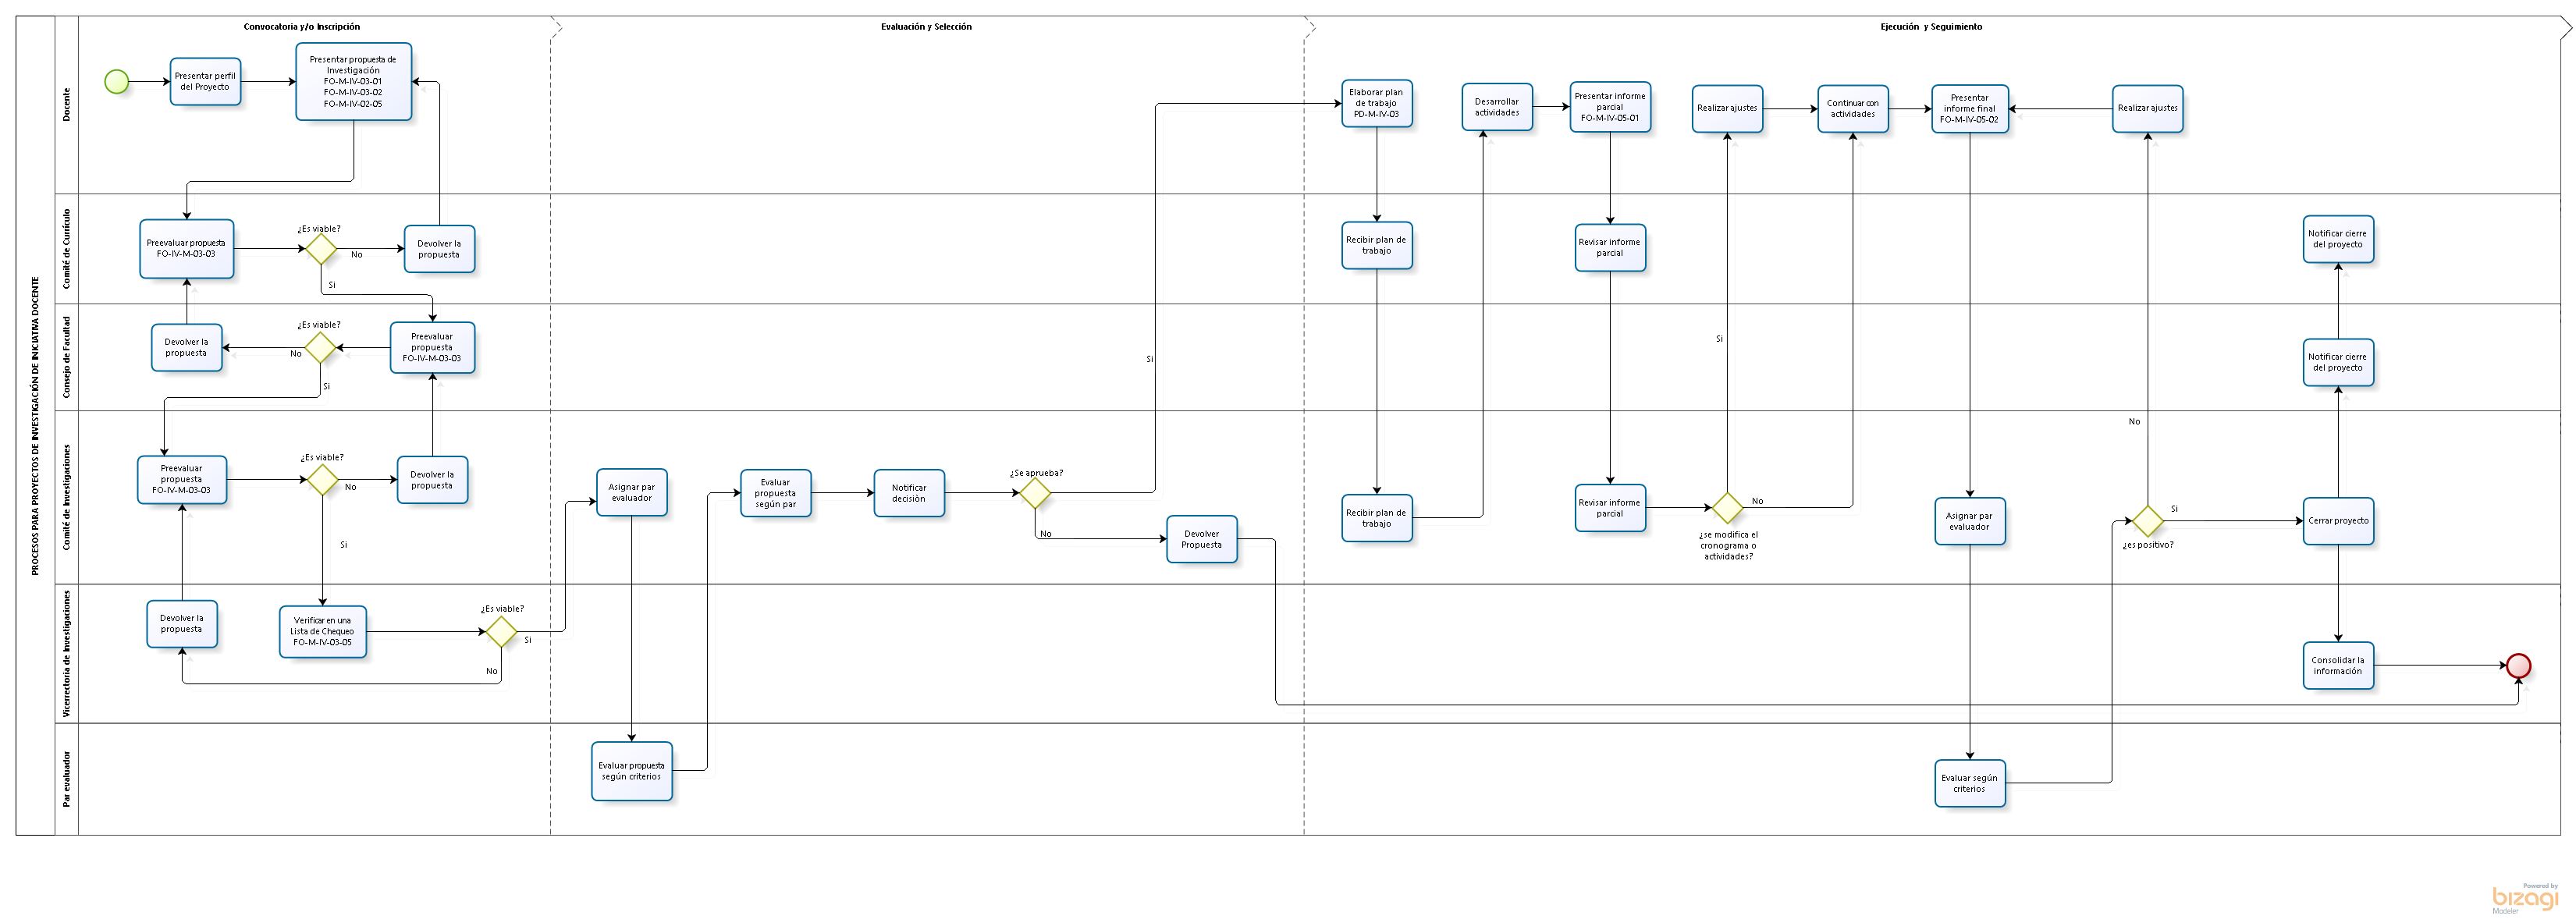
\includegraphics[width=\textwidth]{resources/procesos/PROPUESTO_INICIATIVA_FINAL.PNG} %
\captionof{figure}{Procesos para proyectos de investigaci�n iniciativa docente}
\label{proc_proy_inv_ini_doc}


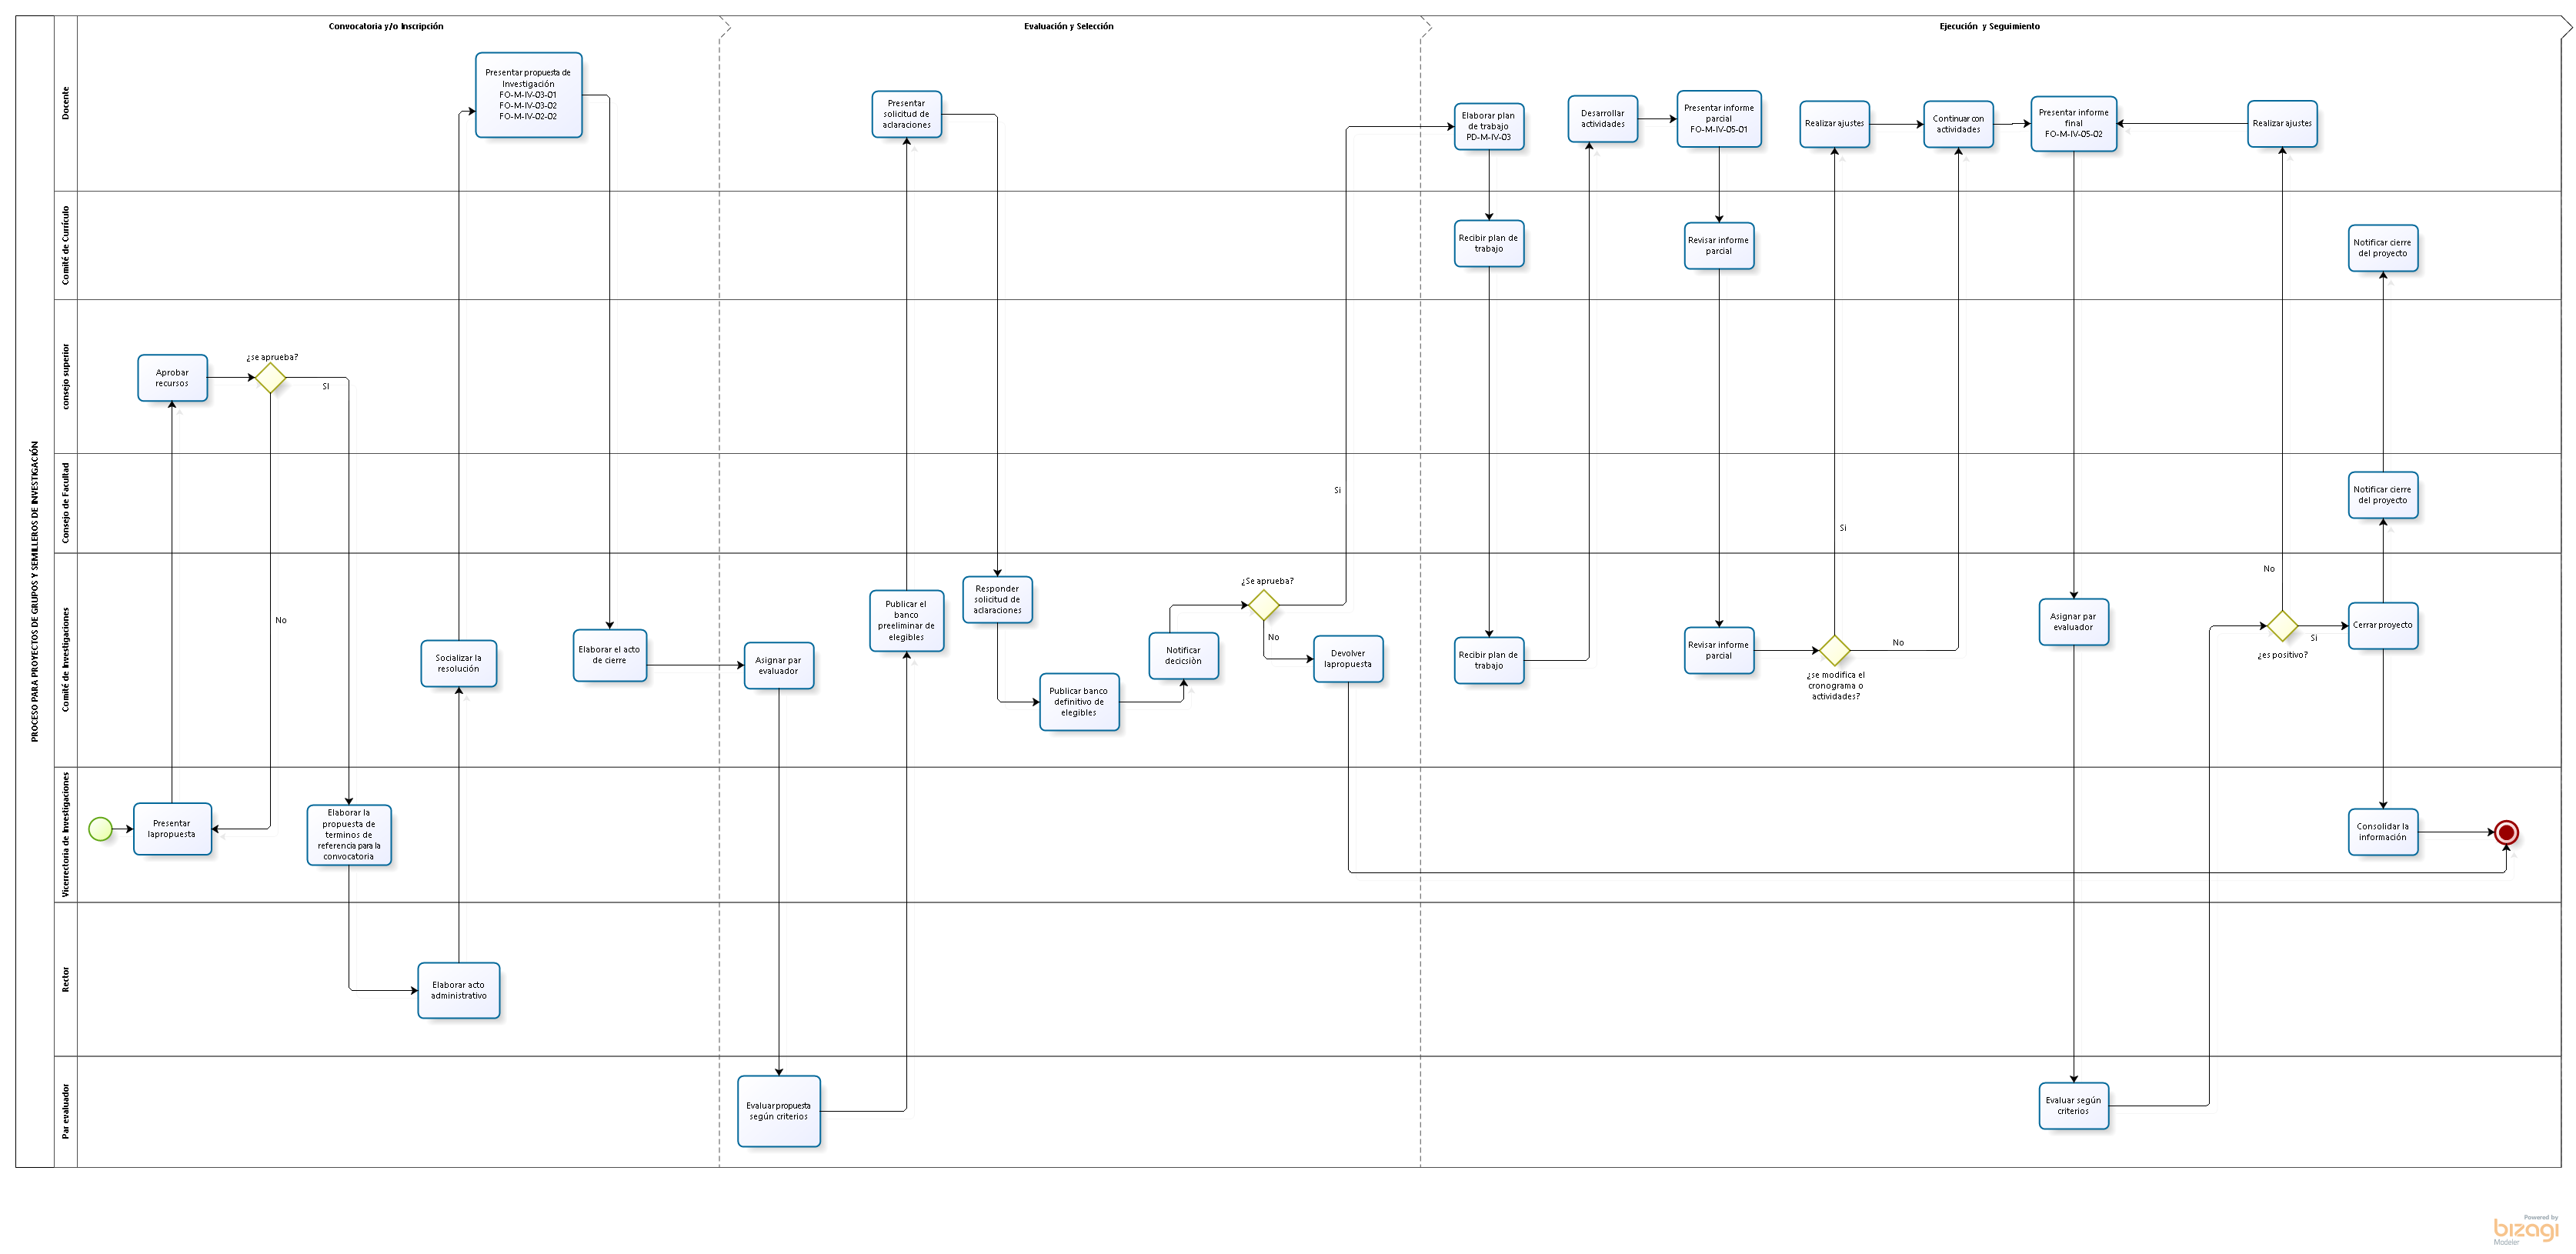
\includegraphics[width=\textwidth]{resources/procesos/PROPUESTO_CONVOCATORIA_FINAL.PNG} %
\captionof{figure}{Procesos para proyectos de grupos y semilleros de investigaci�n}
\label{proc_proy_grup_sem_inv}